\documentclass[aspectratio=169,10pt]{beamer}

% Theme and Color Scheme
\usetheme{Madrid}
\usecolortheme{whale}

\definecolor{rakshakNavy}{RGB}{15, 32, 67}
\definecolor{rakshakSaffron}{RGB}{235, 110, 30}
\definecolor{rakshakGreen}{RGB}{24, 134, 75}
\definecolor{rakshakRed}{RGB}{205, 32, 38}
\definecolor{rakshakGray}{RGB}{245, 247, 250}
\definecolor{rakshakText}{RGB}{33, 37, 41}

\setbeamercolor{palette primary}{bg=rakshakNavy,fg=white}
\setbeamercolor{palette secondary}{bg=rakshakSaffron,fg=white}
\setbeamercolor{palette tertiary}{bg=rakshakNavy,fg=white}
\setbeamercolor{titlelike}{bg=rakshakNavy,fg=white}
\setbeamercolor{block title}{bg=rakshakNavy,fg=white}
\setbeamercolor{block body}{bg=rakshakGray,fg=rakshakText}
\setbeamercolor{block title alerted}{bg=rakshakRed,fg=white}
\setbeamercolor{block body alerted}{bg=rakshakGray,fg=rakshakText}
\setbeamercolor{block title example}{bg=rakshakGreen,fg=white}
\setbeamercolor{block body example}{bg=rakshakGray,fg=rakshakText}

\usepackage{fontspec}
\setsansfont{Nirmala UI}
\setmainfont{Nirmala UI}

\usepackage{booktabs}
\usepackage{amsmath}
\usepackage{tikz}
\usetikzlibrary{shapes,arrows.meta,positioning}

\title[\textbf{Rakshak}: AI Call Guardian]{\textbf{RAKSHAK (रक्षक / રક્ષક)}}
\subtitle{Real-Time AI Guardian Against ``Digital Arrest'', Fake KYC \& Courier Scams}
\author[Team Rakshak]{\textbf{Team Rakshak} \\ Powered by Google Gemini End-to-End Audio \& Vertex AI}
\institute[Hackathon 2026]{Indian Cyber Safety Initiative}
\date{\today}

\begin{document}

% Slide 1: Title
\begin{frame}
  \titlepage
\end{frame}

% Slide 2: The Problem
\begin{frame}{The Crisis: Indian Elders Under ``Digital Arrest''}
\begin{columns}[T]
\column{0.52\textwidth}
\begin{block}{The Anatomy of the Scam}
\begin{itemize}
    \item \textbf{High-Stakes Extortion}: Scammers pose as Mumbai Police, CBI, ED, or FedEx Narcotics wing.
    \item \textbf{Isolation Weapon}: Victims are commanded into a closed room on a continuous video call (``Digital Arrest'').
    \item \textbf{Target Group}: Elders, retirees, and first-time smartphone users who are alone and vulnerable.
    \item \textbf{Scale}: Over \textbf{thousands of crores} looted across India annually.
\end{itemize}
\end{block}

\column{0.45\textwidth}
\begin{alertblock}{Why Victims Comply}
\begin{itemize}
    \item Fear of arrest warrants \& forged Supreme Court summons.
    \item Artificial urgency: ``Transfer to RBI verification account in 15 mins''.
    \item \textbf{The Core Vulnerability}: The victim is \textbf{completely alone on the call} with no one to verify facts.
\end{itemize}
\end{alertblock}
\end{columns}
\end{frame}

% Slide 3: The Rakshak Solution
\begin{frame}{The Solution: Rakshak Silent Co-Pilot}
\begin{block}{How Rakshak Protects in Real-Time}
Rakshak runs as a silent, on-device / edge guardian listening to incoming phone audio in \textbf{5-second sliding chunks}.
\end{block}
\vspace{0.3cm}
\begin{columns}[T]
\column{0.32\textwidth}
\begin{block}{1. Stream Ingestion}
Processes raw 16kHz PCM audio without transcribing to text first; preserves tone, hesitation, and pressure cues.
\end{block}

\column{0.32\textwidth}
\begin{alertblock}{2. Mid-Call Alert}
Flags scams at \textbf{15s--25s}, intervening \textbf{before} the victim hands over bank accounts or OTPs.
\end{alertblock}

\column{0.32\textwidth}
\begin{exampleblock}{3. Vernacular Voice}
Explains the scam in simple, reassuring \textbf{Hindi \& Gujarati}: ``Police never arrest on video call''.
\end{exampleblock}
\end{columns}
\end{frame}

% Slide 4: Gemini Audio vs Web Speech API
\begin{frame}{Why Gemini End-to-End Audio?}
\begin{table}[]
\centering
\small
\begin{tabular}{p{3.8cm} p{5cm} p{5cm}}
\toprule
\textbf{Capability} & \textbf{Browser Web Speech API} & \textbf{Rakshak (Gemini Audio)} \\
\midrule
\textbf{Colloquial Dialects} & Fails on Gujarati/Hindi code-switching & Native comprehension of Gujarati, Hinglish \& regional nuances \\
\midrule
\textbf{Acoustic Robustness} & Severely degrades under phone line noise \& hiss & Trained on raw audio representations; ignores GSM compression \\
\midrule
\textbf{Context Window} & Stateless per phrase & Accumulates session state across all prior chunks \\
\midrule
\textbf{Urgency \& Threat Intonation} & Strips vocal emotion & Detects aggressive caller tone \& psychological pressure \\
\bottomrule
\end{tabular}
\end{table}
\end{frame}

% Slide 5: The Red Flag Taxonomy
\begin{frame}{Precision Scam Taxonomy}
\begin{columns}[T]
\column{0.48\textwidth}
\begin{block}{Decisive Red Flags}
\begin{itemize}
    \item \textbf{authority\_impersonation}: Police, CBI, TRAI, RBI, or FedEx customs officials.
    \item \textbf{threat\_or\_arrest}: Threat of FIR, jail warrant, pension freeze.
    \item \textbf{secrecy\_isolation}: ``Do not disconnect'', ``Do not tell your family''.
    \item \textbf{money\_transfer}: Safe RBI account, clearance fee, UPI transfer.
    \item \textbf{otp\_request}: Demanding OTP, PIN, or CVV.
\end{itemize}
\end{block}

\column{0.48\textwidth}
\begin{alertblock}{Decision Logic}
\begin{itemize}
    \item Single high-confidence flag triggers \textbf{suspicious} status.
    \item Dual category correlation (e.g. \textit{Authority Impersonation} + \textit{Arrest Threat}) triggers \textbf{immediate mid-call intervention}.
    \item Skips follow-up LLM summarization for sub-second latency.
\end{itemize}
\end{alertblock}
\end{columns}
\end{frame}

% Slide 6: Live Validation & Mid-Call Intervention
\begin{frame}{Live Demo Verification (Mid-Call Detection)}
\begin{block}{Timeline of Scripted Digital Arrest Call (\texttt{digital\_arrest\_hi.wav})}
\begin{itemize}
    \item \textbf{0.0s -- 5.0s} [SAFE]: ``Caller asks for Ramesh Patel, confirms identity.''
    \item \textbf{5.0s -- 10.0s} [SUSPICIOUS]: ``Claims to be Inspector Vikram Singh, Mumbai Cyber Crime.''
    \item \textbf{15.0s -- 25.0s} \textbf{\color{rakshakRed}[SCAM ALERT TRIGGERED (100\% Confidence)]}
\end{itemize}
\end{block}

\begin{alertblock}{Generated Vernacular Warnings}
\textbf{हिंदी}: कोई भी असली पुलिस अधिकारी फोन पर गिरफ्तारी की धमकी नहीं देता। फोन तुरंत काट दीजिए। \\
\textbf{ગુજરાતી}: કોઈપણ અસલી પોલીસ અધિકારી ફોન પર ધરપકડની ધમકી નથી આપતા. ફોન તરત જ કાપી નાખો.
\end{alertblock}

\begin{exampleblock}{Outcome}
Alert raised \textbf{35 seconds before} the scammer asked for 4 Lakh rupees!
\end{exampleblock}
\end{frame}

% Slide 7: Zero False Positives
\begin{frame}{Guarantee: Never Cry Wolf}
\begin{columns}[T]
\column{0.48\textwidth}
\begin{exampleblock}{Genuine Call (\texttt{genuine\_gu.wav})}
\textbf{Context}: Son calling his mother in Gujarati regarding dinner and doctor's appointment.
\begin{itemize}
    \item \textbf{0--5s}: Greeted 'mummy', answered 'Ha mummy'.
    \item \textbf{5--10s}: Discussing health \& medicine.
    \item \textbf{10--15s}: Doctor appointment at 10 AM.
    \item \textbf{Verdict}: \textbf{SAFE --- 0 alerts raised}.
\end{itemize}
\end{exampleblock}

\column{0.48\textwidth}
\begin{block}{Contextual Safety Filters}
\begin{itemize}
    \item Delivery callers asking for society gate directions $\rightarrow$ \textbf{SAFE}
    \item Bank automated balances or legit OTP reminder $\rightarrow$ \textbf{SAFE}
    \item Advice like ``never share OTP'' $\rightarrow$ Recognized as a \textbf{protective positive sign}.
\end{itemize}
\end{block}
\end{columns}
\end{frame}

% Slide 8: Cloud Architecture
\begin{frame}{Cloud Native Architecture on Google Cloud}
\begin{center}
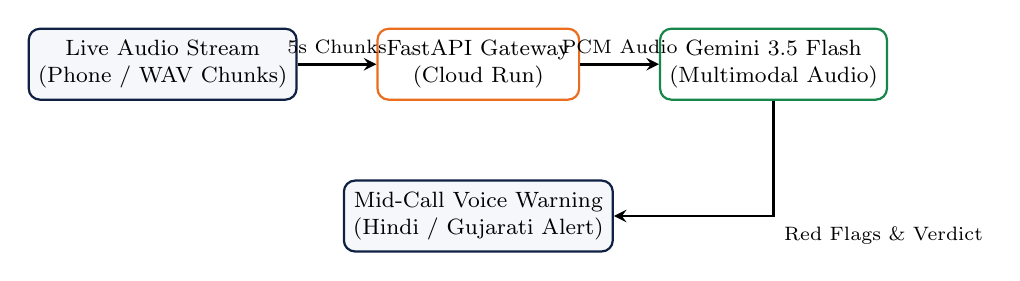
\begin{tikzpicture}[node distance=1.1cm, auto,
    block/.style={rectangle, draw=rakshakNavy, fill=rakshakGray, thick, rounded corners, minimum height=0.9cm, align=center, font=\footnotesize},
    accent/.style={rectangle, draw=rakshakSaffron, fill=white, thick, rounded corners, minimum height=0.9cm, align=center, font=\footnotesize},
    cloud/.style={rectangle, draw=rakshakGreen, fill=white, thick, rounded corners, minimum height=0.9cm, align=center, font=\footnotesize}]

    \node [block] (audio) {Live Audio Stream \\ (Phone / WAV Chunks)};
    \node [accent, right=1.0cm of audio] (fastapi) {FastAPI Gateway \\ (Cloud Run)};
    \node [cloud, right=1.0cm of fastapi] (gemini) {Gemini 3.5 Flash \\ (Multimodal Audio)};
    \node [block, below=1.0cm of fastapi] (alert) {Mid-Call Voice Warning \\ (Hindi / Gujarati Alert)};

    \draw[->, >=stealth, line width=1pt] (audio) -- node[above]{\scriptsize 5s Chunks} (fastapi);
    \draw[->, >=stealth, line width=1pt] (fastapi) -- node[above]{\scriptsize PCM Audio} (gemini);
    \draw[->, >=stealth, line width=1pt] (gemini) |- node[below right]{\scriptsize Red Flags \& Verdict} (alert);
\end{tikzpicture}
\end{center}
\vspace{0.2cm}
\begin{itemize}
    \item \textbf{Google Cloud Run}: Serverless auto-scaling container backend.
    \item \textbf{Vertex AI Global}: Low-latency multimodal audio understanding.
    \item \textbf{A2A Protocol Ready}: Autonomous Agent interoperability.
\end{itemize}
\end{frame}

% Slide 9: Conclusion
\begin{frame}{Summary \& Social Impact}
\begin{block}{Impact for Indian Citizens}
\begin{itemize}
    \item \textbf{Protection for the Most Vulnerable}: Replaces solitude with an intelligent guardian.
    \item \textbf{Linguistic Inclusivity}: Native support for India's regional languages.
    \item \textbf{Actionable Clarity}: Eliminates panic by debunking the lie before money is lost.
\end{itemize}
\end{block}

\vspace{0.4cm}
\begin{center}
\LARGE \textbf{Rakshak: Defending Indian Families from Scams} \\
\vspace{0.2cm}
\normalsize \textit{Questions \& Demonstration}
\end{center}
\end{frame}

\end{document}
